\documentclass[11pt]{article}
\usepackage{minted, tikz}
\usepackage{amsfonts, amssymb, amsmath, float}
\usepackage{enumerate, esint, nicefrac, algorithm2e}
\parindent 0px
\date{November 14, 2023}
\title{CS301 :: Homework 5}
\author{Ryan Magdaleno}

% Helpful ::
% \line(1,0){358px}

\begin{document}
\maketitle

%%%%%%%%%%%%%%%%%%%%%%%%%%%%%%%%%%%%%%%%%%%%%%%%%%%%%%%%%%%%%%%%%%%%%%%%%%%%%%%%%%%%%%%%%

\textbf{Problem 1. Turing Machines}

\begin{enumerate}[a)]
    \item
    Give a \textit{high-level} description of a Turing Machine that decides the
    \\ language:
    $$L = \{0^n1^m \,|\, n\ge 2m\}$$
    \vspace{5px}\textbf{Solution ::}

    $M = $ "On input string $w$:
    \begin{enumerate}[\hspace{15px}1.]
        \item
        If the input string is empty (starts on ' ') then accept, else go to step 2.
        \item
        Scan the input from left to right and make sure that the input is of the form
        "$0^*1^*$", and reject if it isn't.
        \item 
        Return tape head to the front of the input tape.
        \item 
        Move head to the first '1' character on tape.
        \item 
        Repeat the following until head is over a ' ', if so go to step 8.
        \item 
        \hspace{15px}Scan right once and check it is a '1', else reject.
        \item 
        \hspace{15px}Move head right once, go to step 5 loop condition check step.
        \item Return tape head to the front of the input tape and scan right until first
        0.
        \item 
        Repeat the following until no more 1s are on the tape, if no 1s go to step 14.
        \item
        \hspace{15px}Replace the leftmost '0' with a 'x'.
        \item 
        \hspace{15px}Scan right until a '1' occurs. If there are no 1s, reject.
        \item
        \hspace{15px}Replace the leftmost '1' with a 'x'.
        \item 
        \hspace{15px}Return tape head to front end of tape, and go to step 9.
        \item
        Accept."
    \end{enumerate}
    \pagebreak

    \item
    Give a state diagram for the Turing Machine you described in part (a), for the
    language:
    $$L = \{0^n1^m \,|\, n\ge2m\}$$
    \vspace{5px}\textbf{Solution ::}
    \begin{center}
    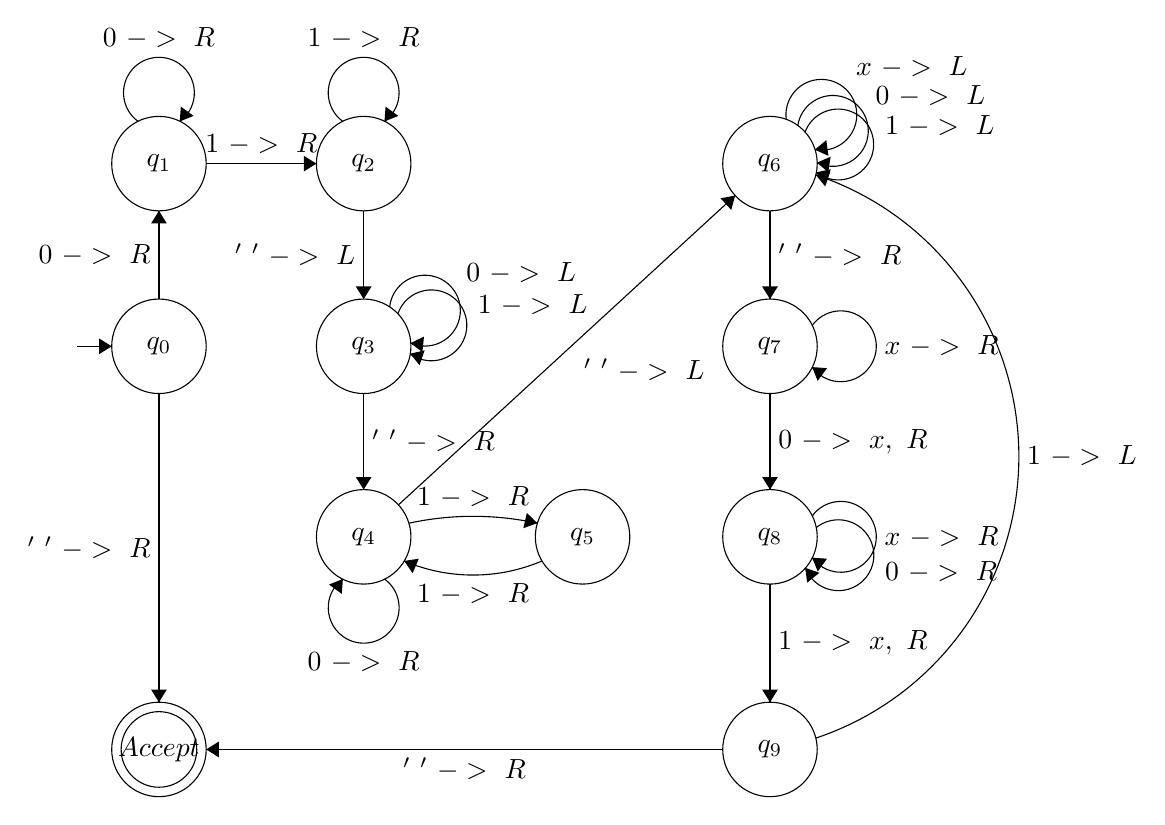
\begin{tikzpicture}[scale=0.2]
    \tikzstyle{every node}+=[inner sep=0pt]
    \draw [black] (15.6,-21.1) circle (3);
    \draw (15.6,-21.1) node {$q_0$};
    \draw [black] (15.6,-9.5) circle (3);
    \draw (15.6,-9.5) node {$q_1$};
    \draw [black] (28.6,-9.5) circle (3);
    \draw (28.6,-9.5) node {$q_2$};
    \draw [black] (28.6,-21.1) circle (3);
    \draw (28.6,-21.1) node {$q_3$};
    \draw [black] (28.6,-33.2) circle (3);
    \draw (28.6,-33.2) node {$q_4$};
    \draw [black] (42.5,-33.2) circle (3);
    \draw (42.5,-33.2) node {$q_5$};
    \draw [black] (54.4,-9.5) circle (3);
    \draw (54.4,-9.5) node {$q_6$};
    \draw [black] (54.4,-21.1) circle (3);
    \draw (54.4,-21.1) node {$q_7$};
    \draw [black] (54.4,-33.2) circle (3);
    \draw (54.4,-33.2) node {$q_8$};
    \draw [black] (54.4,-46.7) circle (3);
    \draw (54.4,-46.7) node {$q_9$};
    \draw [black] (15.6,-46.7) circle (3);
    \draw (15.6,-46.7) node {$Accept$};
    \draw [black] (15.6,-46.7) circle (2.4);
    \draw [black] (10.4,-21.1) -- (12.6,-21.1);
    \fill [black] (12.6,-21.1) -- (11.8,-20.6) -- (11.8,-21.6);
    \draw [black] (15.6,-18.1) -- (15.6,-12.5);
    \fill [black] (15.6,-12.5) -- (15.1,-13.3) -- (16.1,-13.3);
    \draw (15.1,-15.3) node [left] {$0\mbox{ }->\mbox{ }R$};
    \draw [black] (14.277,-6.82) arc (234:-54:2.25);
    \draw (15.6,-2.25) node [above] {$0\mbox{ }->\mbox{ }R$};
    \fill [black] (16.92,-6.82) -- (17.8,-6.47) -- (16.99,-5.88);
    \draw [black] (18.6,-9.5) -- (25.6,-9.5);
    \fill [black] (25.6,-9.5) -- (24.8,-9) -- (24.8,-10);
    \draw (22.1,-9) node [above] {$1\mbox{ }->\mbox{ }R$};
    \draw [black] (27.277,-6.82) arc (234:-54:2.25);
    \draw (28.6,-2.25) node [above] {$1\mbox{ }->\mbox{ }R$};
    \fill [black] (29.92,-6.82) -- (30.8,-6.47) -- (29.99,-5.88);
    \draw [black] (28.6,-12.5) -- (28.6,-18.1);
    \fill [black] (28.6,-18.1) -- (29.1,-17.3) -- (28.1,-17.3);
    \draw (28.1,-15.3) node [left] {$'\mbox{ }'\mbox{ }->\mbox{ }L$};
    \draw [black] (28.6,-24.1) -- (28.6,-30.2);
    \fill [black] (28.6,-30.2) -- (29.1,-29.4) -- (28.1,-29.4);
    \draw (29.1,-27.15) node [right] {$'\mbox{ }'\mbox{ }->\mbox{ }R$};
    \draw [black] (30.251,-18.609) arc (174.18741:-113.81259:2.25);
    \draw (35.09,-16.47) node [right] {$0\mbox{ }->\mbox{ }L$};
    \fill [black] (31.58,-20.9) -- (32.33,-21.47) -- (32.43,-20.48);
    \draw [black] (31.469,-32.335) arc (102.29299:77.70701:19.166);
    \fill [black] (39.63,-32.33) -- (38.96,-31.68) -- (38.74,-32.65);
    \draw (35.55,-31.4) node [above] {$1\mbox{ }->\mbox{ }R$};
    \draw [black] (39.931,-34.731) arc (-66.89907:-113.10093:11.166);
    \fill [black] (31.17,-34.73) -- (31.71,-35.51) -- (32.1,-34.59);
    \draw (35.55,-36.13) node [below] {$1\mbox{ }->\mbox{ }R$};
    \draw [black] (29.923,-35.88) arc (54:-234:2.25);
    \draw (28.6,-40.45) node [below] {$0\mbox{ }->\mbox{ }R$};
    \fill [black] (27.28,-35.88) -- (26.4,-36.23) -- (27.21,-36.82);
    \draw [black] (30.81,-31.17) -- (52.19,-11.53);
    \fill [black] (52.19,-11.53) -- (51.26,-11.7) -- (51.94,-12.44);
    \draw (46.41,-21.84) node [below] {$'\mbox{ }'\mbox{ }->\mbox{ }L$};
    \draw [black] (55.433,-6.696) arc (187.50605:-100.49395:2.25);
    \draw (59.83,-3.38) node [right] {$x\mbox{ }->\mbox{ }L$};
    \fill [black] (57.25,-8.61) -- (58.11,-9.01) -- (57.98,-8.01);
    \draw [black] (56.166,-7.09) arc (171.4952:-116.5048:2.25);
    \draw (61.07,-5.24) node [right] {$0\mbox{ }->\mbox{ }L$};
    \fill [black] (57.39,-9.44) -- (58.1,-10.05) -- (58.25,-9.06);
    \draw [black] (56.624,-7.504) arc (159.65013:-128.34987:2.25);
    \draw (61.67,-7.13) node [right] {$1\mbox{ }->\mbox{ }L$};
    \fill [black] (57.34,-10.05) -- (57.91,-10.8) -- (58.26,-9.86);
    \draw [black] (54.4,-12.5) -- (54.4,-18.1);
    \fill [black] (54.4,-18.1) -- (54.9,-17.3) -- (53.9,-17.3);
    \draw (54.9,-15.3) node [right] {$'\mbox{ }'\mbox{ }->\mbox{ }R$};
    \draw [black] (54.4,-24.1) -- (54.4,-30.2);
    \fill [black] (54.4,-30.2) -- (54.9,-29.4) -- (53.9,-29.4);
    \draw (54.9,-27.15) node [right] {$0\mbox{ }->\mbox{ }x,\mbox{ }R$};
    \draw [black] (57.08,-19.777) arc (144:-144:2.25);
    \draw (61.65,-21.1) node [right] {$x\mbox{ }->\mbox{ }R$};
    \fill [black] (57.08,-22.42) -- (57.43,-23.3) -- (58.02,-22.49);
    \draw [black] (57.08,-31.877) arc (144:-144:2.25);
    \draw (61.65,-33.2) node [right] {$x\mbox{ }->\mbox{ }R$};
    \fill [black] (57.08,-34.52) -- (57.43,-35.4) -- (58.02,-34.59);
    \draw [black] (57.331,-32.618) arc (128.95719:-159.04281:2.25);
    \draw (61.68,-35.46) node [right] {$0\mbox{ }->\mbox{ }R$};
    \fill [black] (56.64,-35.17) -- (56.76,-36.11) -- (57.54,-35.48);
    \draw [black] (30.769,-19.045) arc (161.18571:-126.81429:2.25);
    \draw (35.82,-18.47) node [right] {$1\mbox{ }->\mbox{ }L$};
    \fill [black] (31.55,-21.57) -- (32.15,-22.3) -- (32.47,-21.36);
    \draw [black] (54.4,-36.2) -- (54.4,-43.7);
    \fill [black] (54.4,-43.7) -- (54.9,-42.9) -- (53.9,-42.9);
    \draw (54.9,-39.95) node [right] {$1\mbox{ }->\mbox{ }x,\mbox{ }R$};
    \draw [black] (57.31,-10.218) arc (71.57461:-71.57461:18.848);
    \fill [black] (57.31,-10.22) -- (57.91,-10.95) -- (58.23,-10);
    \draw (70.7,-28.1) node [right] {$1\mbox{ }->\mbox{ }L$};
    \draw [black] (51.4,-46.7) -- (18.6,-46.7);
    \fill [black] (18.6,-46.7) -- (19.4,-47.2) -- (19.4,-46.2);
    \draw (35,-47.2) node [below] {$'\mbox{ }'\mbox{ }->\mbox{ }R$};
    \draw [black] (15.6,-24.1) -- (15.6,-43.7);
    \fill [black] (15.6,-43.7) -- (16.1,-42.9) -- (15.1,-42.9);
    \draw (15.1,-33.9) node [left] {$'\mbox{ }'\mbox{ }->\mbox{ }R$};
    \end{tikzpicture}
    \end{center}
\end{enumerate}



\pagebreak

%%%%%%%%%%%%%%%%%%%%%%%%%%%%%%%%%%%%%%%%%%%%%%%%%%%%%%%%%%%%%%%%%%%%%%%%%%%%%%%%%%%%%%%%%

\textbf{Problem 2. Decidable Languages}

Recall that to show a language is decidable, you must show either a \\halting algorithm
which decides it, or a halting recution to a known decidable problem. In either case,
\textbf{you must show that either the algorithm or the reduction halts.}

\vspace{10px}Show that the language $ALL_{DFA}=\{\langle D\rangle \,|\, D$
is a DFA and $L(D)=\sum^*$$\}$ \textit{You may use any problem we have shown to be
decidable in lecture for a reduction.}

\vspace{5px}\textbf{Solution ::}

Algorithm / machine using $E_{DFA}$:

$M = $ "On input $\langle D\rangle$:
\begin{enumerate}[\hspace{15px}1.]
    \item
    Construct a new DFA $A$ such that the language of $A$, $L(A)$ is the
    complement of $L(D)$.
    \item
    Use a TM $T$ that decides $E_{DFA}$ on input $\langle A\rangle$.
    \item 
    Accept if $T$ accepts, else reject.
\end{enumerate}
\end{document}